\subsection{Casos de test}

Para comenzar el análisis sobre el tiempo de ejecución de cada uno de los métodos, decidimos inicialmente estudiar cómo se comportan frente a los test de la cátedra. %A partir de los resultados logramos obtener mayor claridad sobre cómo se desenvuelven. 
%Esto nos permitirá desarrollar una intuición para realizar un estudio más profundo.

\vspace{2em}
\noindent\textsc{Metodología}. Se realizó el cálculo de \textit{PageRank} sobre la implementación que utiliza la \textit{eliminación gaussiana}, con $\varepsilon = 10^{-6}$, y se calculó $||x - pagerank(g, p)||_1$ donde $x$ refiere a la solución verdadera provista por cada uno de los tests. Cabe destacar que este es un proceso determinístico. 

A partir de este resultado realizamos una búsqueda de la tolerancia ideal, para el \textit{método de Jacobi} y el \textit{método de Gauss-Seidel}, que nos permita calcular un resultado de \textit{PageRank} con un error similar al obtenido anteriormente. Para esto, se realizo un binary-search donde en cada paso alteramos la tolerancia $t$ y calculamos el resultado de \textit{PageRank} en base a ambos métodos. Editamos los límites de la tolerancia acorde a si el error calculado fue mayor o menor al error que se cometió con la \textit{eliminación gaussiana}. %Al finalizar este procedimiento obtuvimos tolerancias tales que, al calcular el error de comparar las respuestas que conceden \textit{Jacobi} y \textit{Gauss-Seidel} con la original, sea similar, en orden de magnitud, al error entre la respuesta que retorna PageRank y la original. 

%De este modo se espera realizar una comparación de tiempo de ejecución justa, donde todos los métodos obtengan una respuesta comparable en términos del error cometido.

\vspace{1em}
Dados estos parámeteros, se procedió a calcular \textit{PageRank} para cada test, sobre cada implementación y medir el tiempo de ejecución de la etapa de resolución del sistema lineal asociado. Repetimos este paso diez veces para atenuar las fluctuaciones de tiempo de ejecución. 

\vspace{2em}
\noindent \textsc{Resultados}. Procedemos a detallar los resultados en la Figura (\ref{tiempo_ej}.). 

\begin{figure}[!htbp]
    %\ContinuedFloat
    \centering
    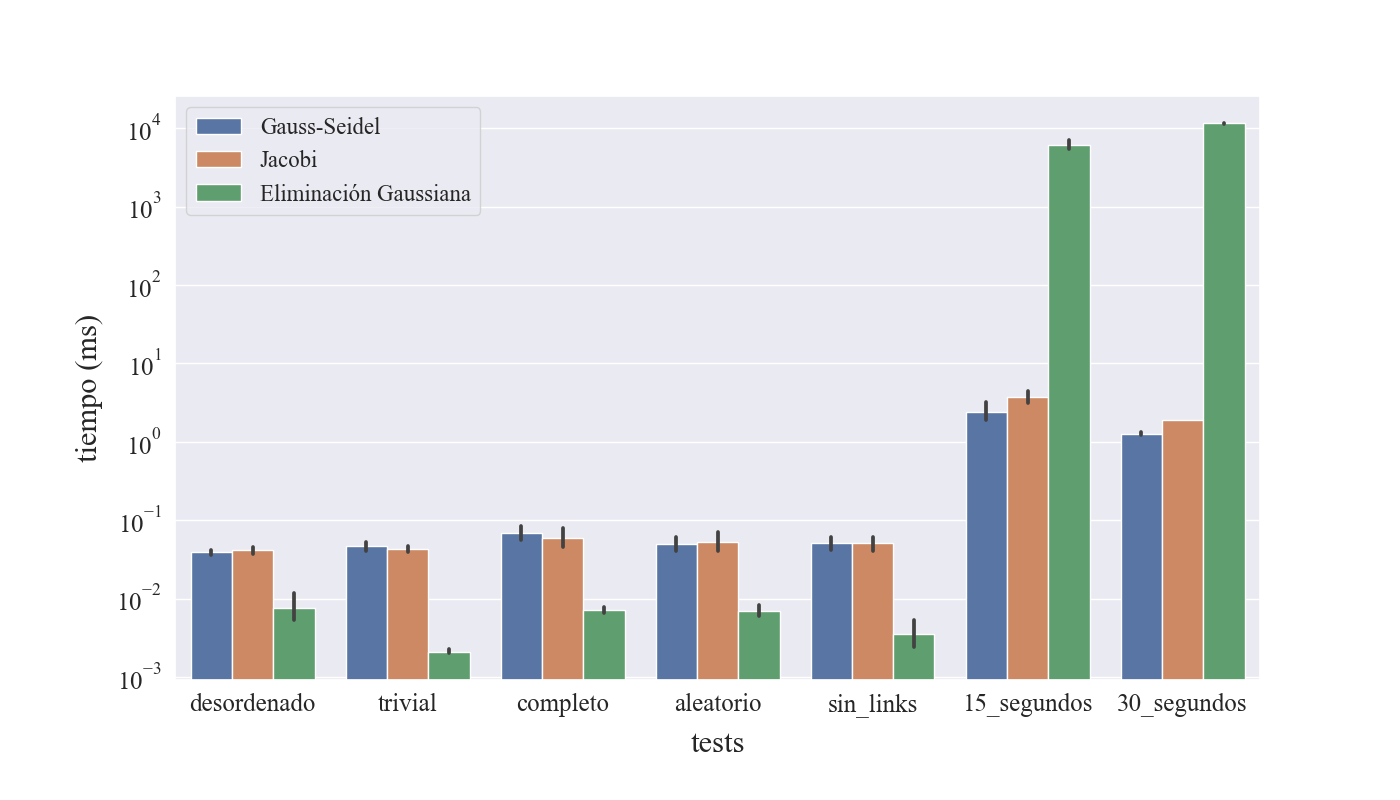
\includegraphics[width=1\textwidth, trim=0 0 0 30]{files/src/.media/tiempo-ejecucion.png}
    \caption{Tiempo de ejecución ---en milisegundos--- de las distintas implementaciones de \textit{PageRank} para cada uno de los tests de la cátedra (escala logarítmica).} \label{tiempo_ej}
\end{figure}


\vspace{1em}
Como se puede apreciar en el gráfico, el \textit{método de Gauss-Seidel} y el \textit{método de Jacobi} son considerablemente más rápidos cuando el tamaño de la matriz es grande. Para el test \textit{30\_segundos}, estos métodos tardaron alrededor de dos milisegundos, mientras que la \textit{eliminación gaussiana} tardó mas de ocho segundos. Sin embargo, cuando el tamaño de la matriz es chico, notamos que la \textit{eliminación gaussiana} es más rápida. 

Por su parte, los métodos iterativos tienen una velocidad muy similar. El \textit{método de Gauss-Seidel} fue apenas más rápido que el \textit{método de Jacobi} en todos los casos evaluados.


% DENSIDADES
\vspace{2em}
\subsection{En función de la densidad del grafo de entrada}
